\subsection{Basic History}
    In 1959, Moore, Edward F. presented one of the first shortest path through a maze algorithm
    \cite{MooreRef}, after a couple of years in 1961 Lee, C. Y. presented the idea of simulating the 
    board wiring on electronics board as a Maze \cite{LeeRef}. Starting from there the idea of Lee Maze
    has been revisited many times, in 1983 Hightower, D. made more contribution to the idea such that
    using modern computers and virtual memories we can mimic the routing problem precisely providing 
    different techniques \cite{HightowerRef}.

\subsection{Router Problem Anatomy}
    The Routing problem has many sections and subsections, in this paper we are mainly concerned with
    Detailed routing. Detailed routing is divided into many subsections, as you can see in fig.\ref{fig:routing_anat} 
    and we are exploring Maze and Line Search subsections.

    \begin{figure}[H]
        \centering
        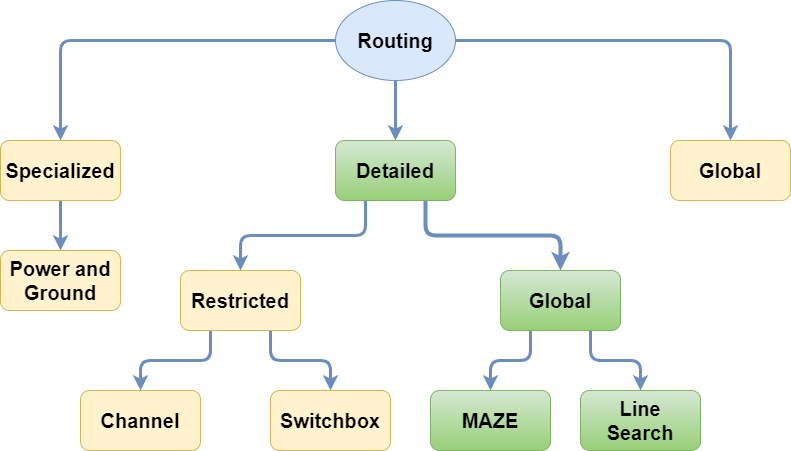
\includegraphics[width=0.4\textwidth]{figures/routing_anatomy.png}
        \caption{Anatomy of various routing techniques.}
        \label{fig:routing_anat}
    \end{figure}

    In the next section we are showing how various algorithms work, and discussing three 
    algorithms, first the \nameref{LeeSection} it's a Maze based algorithm, second the 
    \nameref{MikamiSection} it's a Line-Probe algorithm, and finally the \nameref{SteinerSection} 
    it's a baseline algorithm.

\subsection{Simulation environment}
    Rapidly we'll describe our Simulation's properties:
    \begin{itemize}
        \item Detailed routing (not global)
        \item System is presented as $3D$ Grid,$[D, W, H]$
        \begin{itemize}
            \item D: number of layers 
            \item W: width of each grid
            \item H: height of each grid
        \end{itemize}
        \item Only one source exist as a start.
        \item Multiple targets exist (nested), fan-out.          
        \item Consistent Cost: no bending cost, no extra cost due to vias.
        \item Vias cost is $1$.
        \item Within the same 2D grid path could be horizontally or/and vertically
            chosen.
    \end{itemize}

\subsection{Explored Techniques}
    Before diving into these algorithms make sure to read the \nameref{terminologySection} section first.
    \newline

    \subsubsection{\underline{Lee algorithm}}
    \label{LeeSection}
    This is one of the most common and origin routing algorithms \cite{LeeRef}.

    If there's a path between source $S$ and some target $T$, the algorithm will definitely find it,
    and in case of consistent cost (i.e. no variable cost) the algorithm will not only find the 
    a path but also the shortest one.

    It uses BFS (breadth-first search) to connect targets with the source.

    It works appropriately with multiple layers (i.e. where vias exist).

    The algorithm has three main stages:
    \begin{itemize}
        \item Expansion
        \item Back-tracking
        \item Clean up
    \end{itemize}

    The \textit{Expansion} stage fig \ref{fig:expansionStage} creates like a \textit{halo} shape around the source,
    and it gets larger and the cost of each cell is incremented,
    unless there's an obstacle (block cell),
    until it hits a target and terminates,
    if the expansion reached it's limit with no target hit, this means that the target/s is/are not
    reachable.
% TODO: since the [H] forces the graph to be placed after that section
% extra spacing occur
% so when you are finished with everything..make sure it looks good
    \begin{figure}
        \centering

        \begin{subfigure}[b]{0.3\linewidth}
            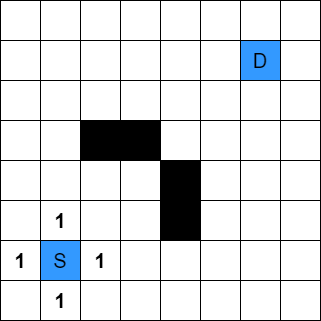
\includegraphics[width=\linewidth]{figures/Lee Stages/grid.png}
            \caption{itr 1}
        \end{subfigure}
        \begin{subfigure}[b]{0.3\linewidth}
            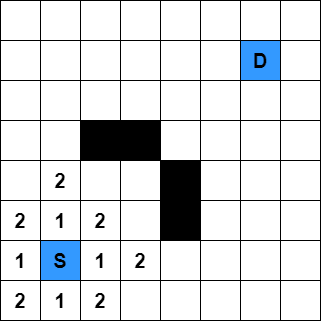
\includegraphics[width=\linewidth]{figures/Lee Stages/grid 1.png}
            \caption{itr 2}
        \end{subfigure}
        \begin{subfigure}[b]{0.3\linewidth}
            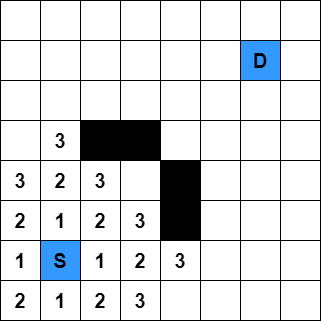
\includegraphics[width=\linewidth]{figures/Lee Stages/grid 2.png}
            \caption{itr 3}
        \end{subfigure}
        \begin{subfigure}[b]{0.3\linewidth}
            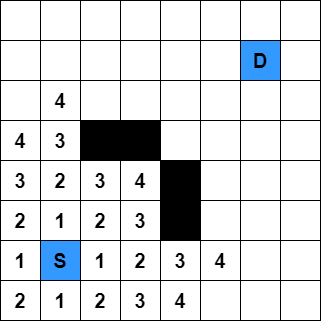
\includegraphics[width=\linewidth]{figures/Lee Stages/grid 3.png}
            \caption{itr 4}
        \end{subfigure}
        \begin{subfigure}[b]{0.3\linewidth}
            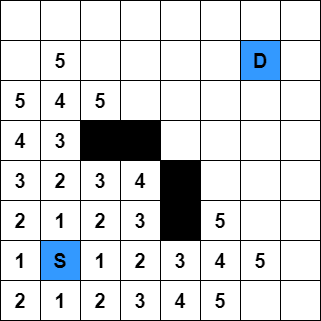
\includegraphics[width=\linewidth]{figures/Lee Stages/grid 4.png}
            \caption{itr 5}
        \end{subfigure}
        \begin{subfigure}[b]{0.3\linewidth}
            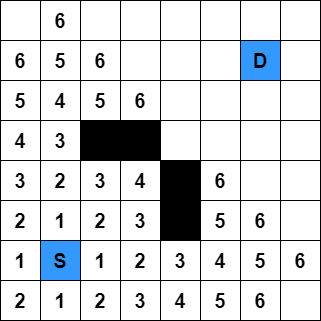
\includegraphics[width=\linewidth]{figures/Lee Stages/grid 5.png}
            \caption{itr 6}
        \end{subfigure}
        \begin{subfigure}[b]{0.3\linewidth}
            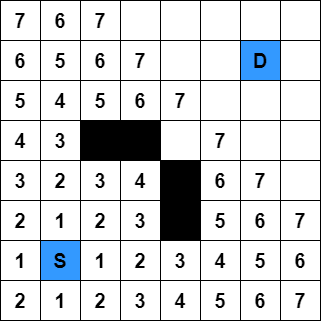
\includegraphics[width=\linewidth]{figures/Lee Stages/grid 6.png}
            \caption{itr 7}
        \end{subfigure}
        \begin{subfigure}[b]{0.3\linewidth}
            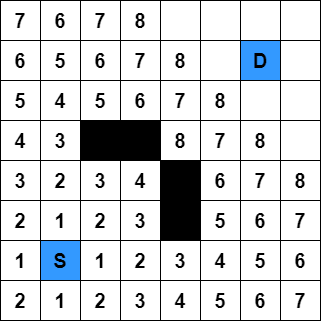
\includegraphics[width=\linewidth]{figures/Lee Stages/grid 7.png}
            \caption{itr 8}
        \end{subfigure}
        \begin{subfigure}[b]{0.3\linewidth}
            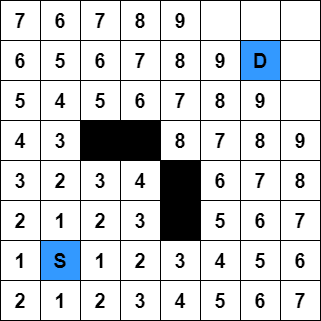
\includegraphics[width=\linewidth]{figures/Lee Stages/grid 8.png}
            \caption{itr 9}
        \end{subfigure}
        \begin{subfigure}[b]{0.3\linewidth}
            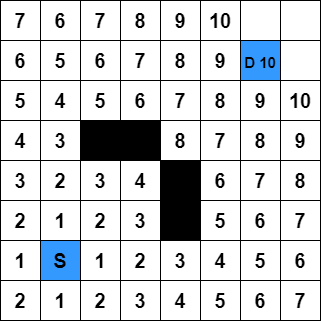
\includegraphics[width=\linewidth]{figures/Lee Stages/grid 9.png}
            \caption{itr 10}
        \end{subfigure}
        
        \caption{Expansion Stage}
        \label{fig:expansionStage}
      \end{figure}
      

    The \textit{Back-tracking} stage fig.\ref{fig:backtrackingStage} gets the path from the target $T$
    to the source $S$.
    Since we are dealing with consistent cost, then the backtracking stage is not that much of an issue
    all we have to do is to decrement the cost by $1$ from the target, until we reach the source.
    In other versions where inconsistent cost exist, and the cost of the path is the total length of it.
    \textbf{Data structure} such as \textbf{priority queue} is used to \textit{pop-up}
    the cell with minimum cost.

    \begin{figure}[H]
        \centering
        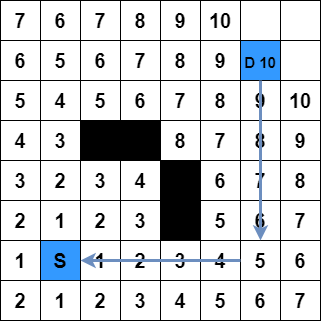
\includegraphics[width=0.35\textwidth]{figures/Lee Stages/back-track.png}
        \caption{Back-tracking Stage}
        \label{fig:backtrackingStage}
    \end{figure}
    The \textit{Clean up} stage fig.\ref{fig:cleanUpStage} converts the path from the source
    to the target into obstacles (blocks) so that no interference between paths may exist.
    and then starts to connect another target to the source with that path of obstacles added.

    \begin{figure}[H]
        \centering
        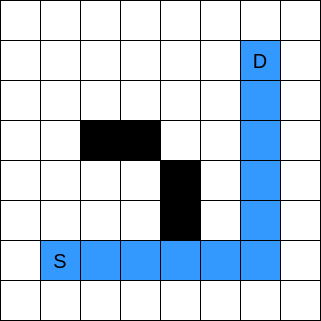
\includegraphics[width=0.35\textwidth]{figures/Lee Stages/clean_up.png}
        \caption{Clean up Stage}
        \label{fig:cleanUpStage}
    \end{figure}

    \subsubsection{\underline{Mikami-Tabuchi algorithm}}
    \label{MikamiSection}
    Mikami-Tabuchi developed the algorithm named after them \cite{mikami1968computer} to address the issues of Lee maze solver, which is the huge requirements of time and space.

Mikami-Tabuchi is simple, fast, low on memory resources but it doesn't guarantee finding the optimal path. It only guarantee finding a path if exists.

Mikami-Tabuchi algorithm is sometimes referred to as \textit{line-probing algorithm} or \textit{line-search algorithm}.

Mikami-Tabuchi basic idea is to extend horizontal and vertical lines/probes from source and target. The algorithm extends those lines until they either hit an edge of the area or an obstacle.

If one of the lines of the source intersected with one of the lines of the target, the algorithm backtracks from the point of intersection to both source and target, and that's the solution.

\begin{figure}[H]
    \centering
    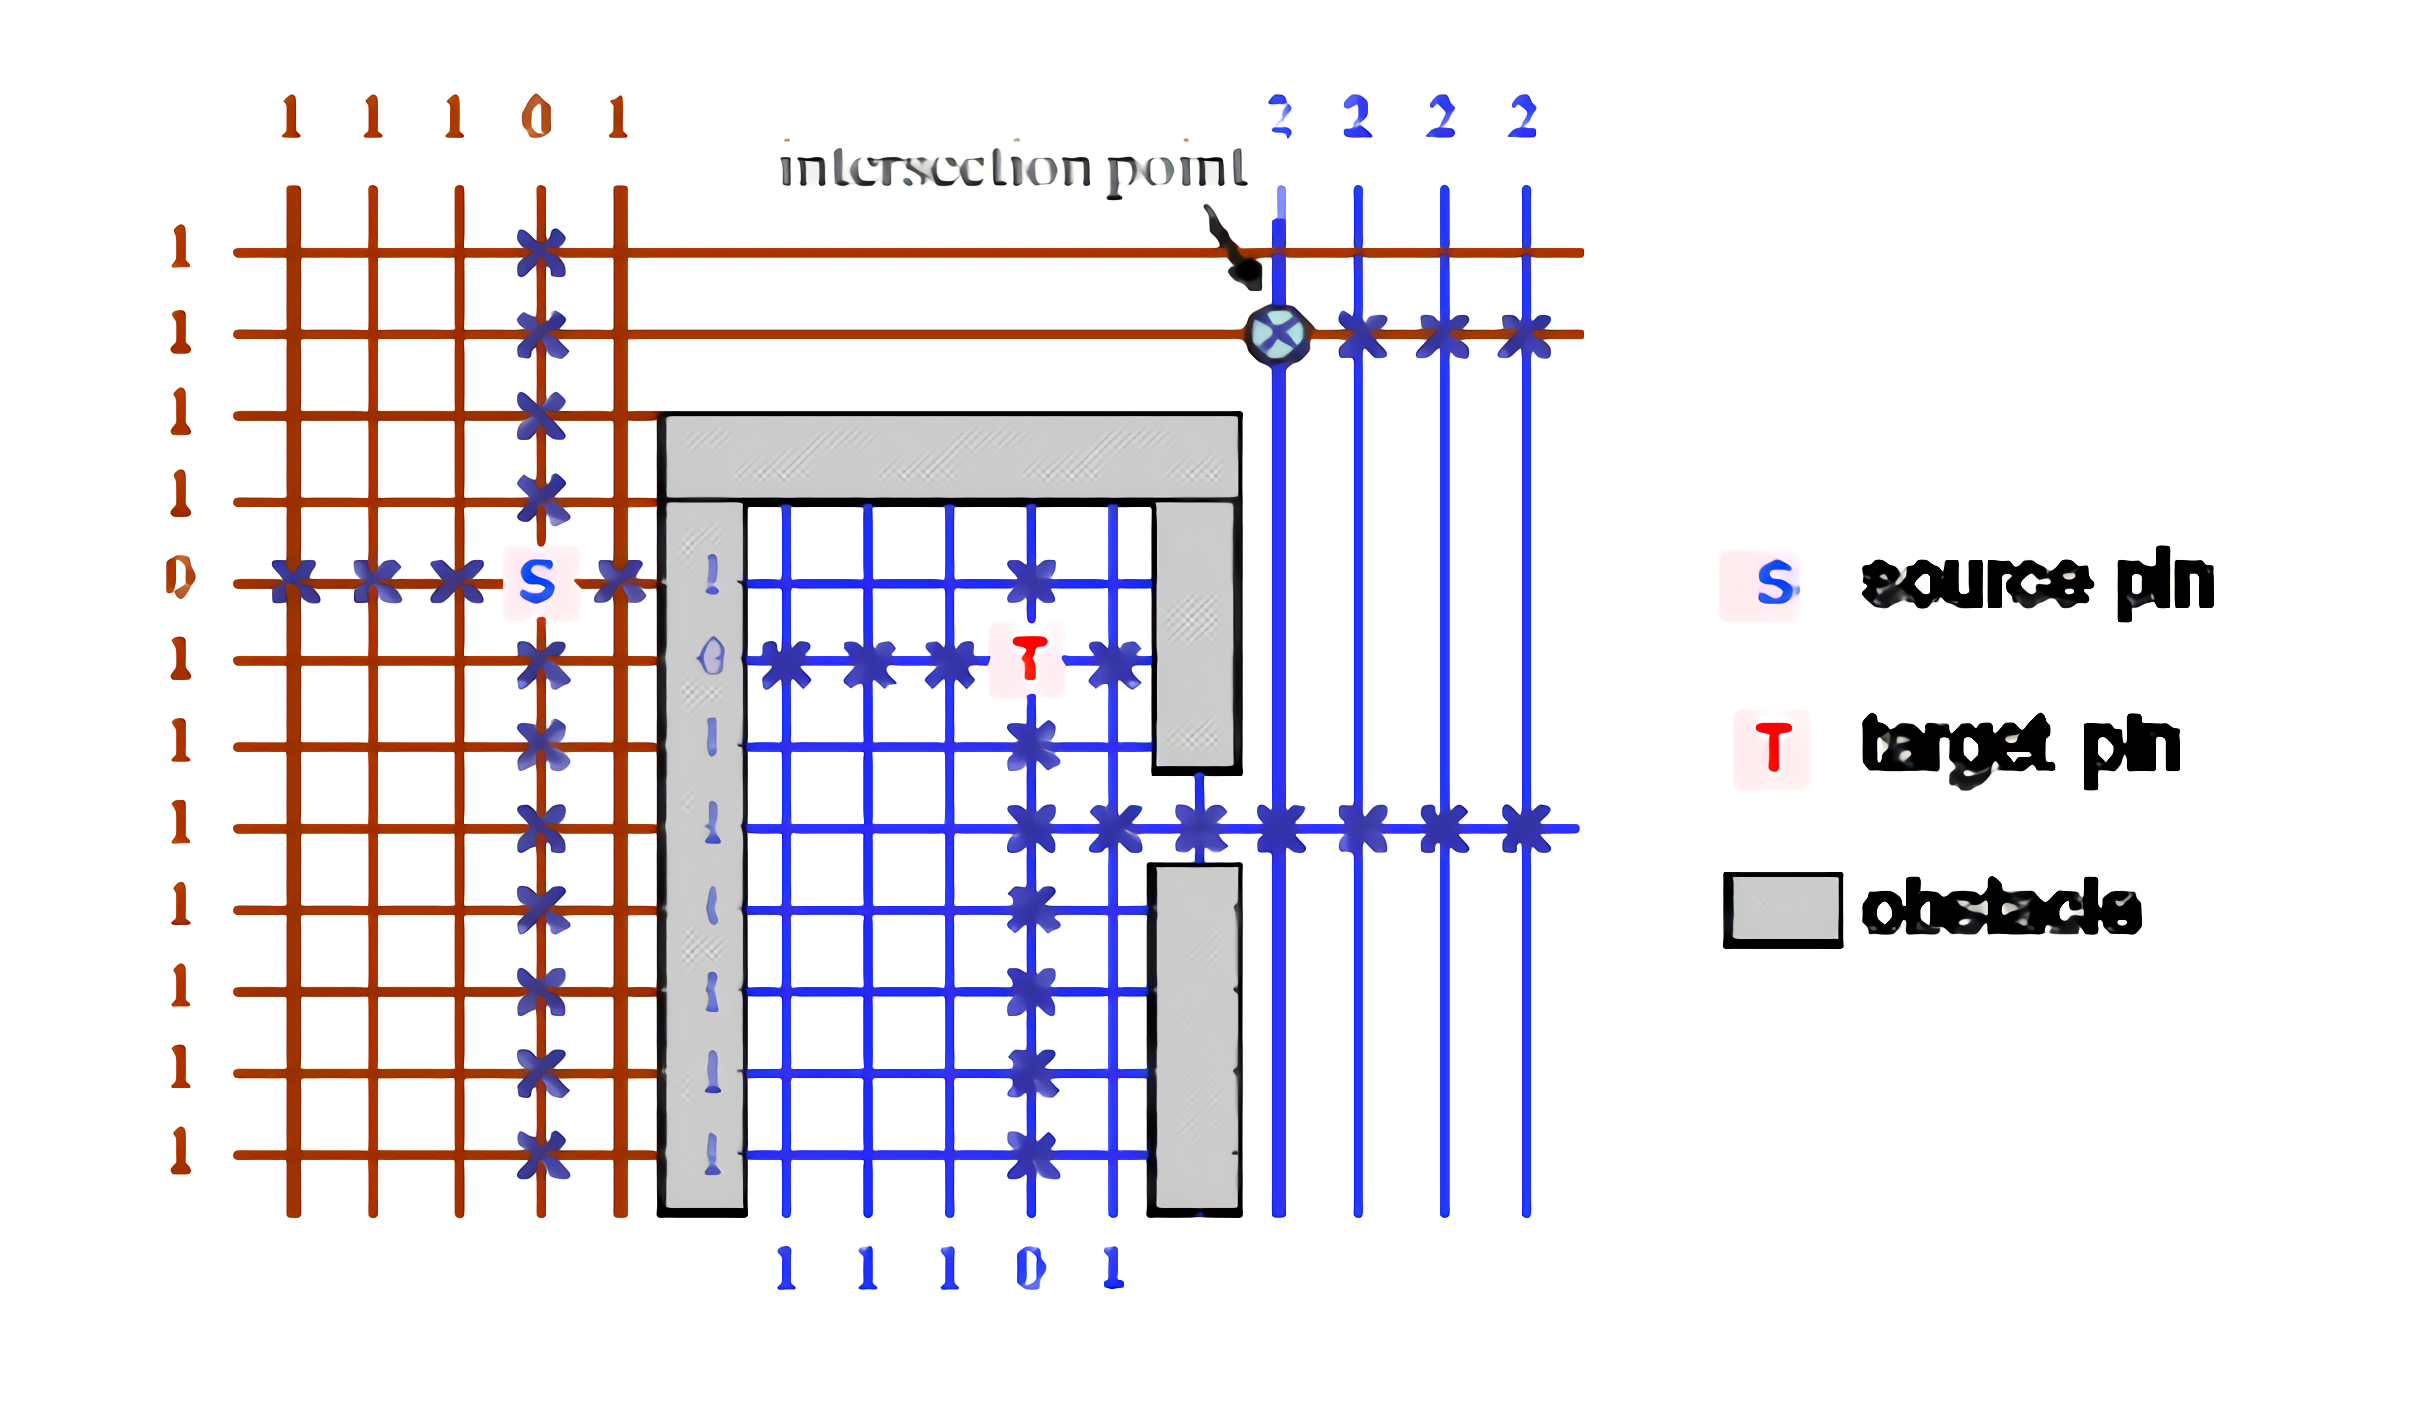
\includegraphics[width=\linewidth]{figures/mikami.png}
    \caption{Mikami Algorithm Illustration \cite{chen2009global}}
    \label{fig:mikamiIllustr}
\end{figure}

Mikami-Tabuchi algorithm wasn't designed with multi-layer in mind. But it could be extended to work with multi-layers by using 3d probes/lines and representing the VIAs as lines that's perpendicular to the layer. If a line in the layer intersected with the VIA line, the algorithm, recursively, extends a probe on the same point but on the other layer.

\begin{algorithm}[h]
\SetAlgoLined
\KwResult{Some path between source and destination.}
    Let S and T be a pair source and destination respectively\;
    Generate 4 lines (2 horizontal and 2 vertical) passing through S and T\;
    Extend these lines till they hit obstacles or the boundary of the layout\;
    \If{a line generated from S intersects a line generated from T}{
        backtrack to find path\;
        return path\;
    }
    $i \leftarrow 1$\;
    \While{no new lines were created}{
        \ForEach{line L $\in$ level $i-1$}{%
            \ForEach{Point p $\in$ line L}{%
                Generate a perpendicular line L2\;
                Extend line L2 till it hit obstacles or the boundary of the layout or intersects with other line L3, where $L3 \in level j$ and $j > 0$\;
                \If{L2 intersects with L3 and L2 and L3 are from different terminals}{%
                    backtrack to find path\;
                    return path\;
                }
            }
        }
        $i \leftarrow i+1$
    }
    \caption{Mikami-Tabuchi Algorithm for Automatic Routing \cite{mikamiPresent}}
\end{algorithm}


    \vspace{1cm}
    \subsubsection{\underline{Steiner algorithm}}
    \label{SteinerSection} is the baseline algorithm for our work.

    The definition of Steiner Tree is very general, we are mainly concerned with minimum Steiner tree problem,
    and it's algorithm.

    Minimum Steiner Tree $(MST)$ algorithm provides the minimum spanning tree that may exist in the graph,
    so that it connects multiple points with each others, using intermediate points called Steiner Points.

    It's basic idea is that, after including the first path step 1 in fig.\ref{fig:steinerStages} 
    -the shortest/closest target to the source-
    any other target that will be connected to the source may be connected to any point of the 
    extracted path, so that it could be connected to the main source or any Steiner Point that's being produced (Grey cells),
    and to connect that target, we need to know which of the left (untaken) targets has the minimum distance to the source
    or any of the Steiner Points as shown in step 2 in fig.\ref{fig:steinerStages}, 
    then pick the one with the minimum cost, step 3 in fig.\ref{fig:steinerStages},
    and that's what makes time grows exponentially.


    \begin{figure}
        \centering

        \begin{subfigure}[b]{0.3\linewidth}
            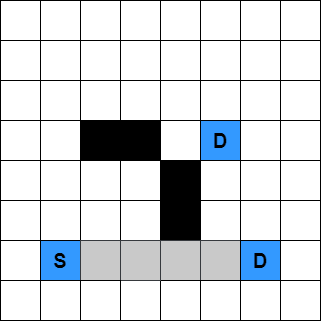
\includegraphics[width=\linewidth]{figures/Steiner Stages/steiner_1.png}
            \caption{step 1}
        \end{subfigure}
        \begin{subfigure}[b]{0.3\linewidth}
            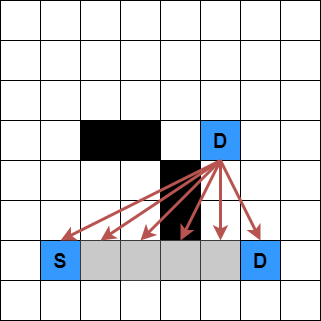
\includegraphics[width=\linewidth]{figures/Steiner Stages/steiner_2.png}
            \caption{step 2}
        \end{subfigure}
        \begin{subfigure}[b]{0.3\linewidth}
            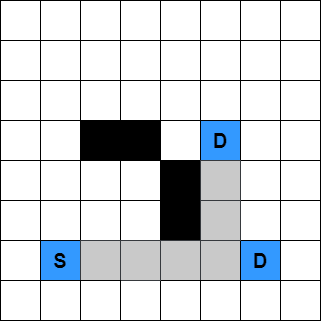
\includegraphics[width=\linewidth]{figures/Steiner Stages/steiner_3.png}
            \caption{step 3}
        \end{subfigure}

        \caption{Steiner Process}
        \label{fig:steinerStages}
    \end{figure}

    As mentioned before, Steiner always provide the optimal path -whenever it exists-,
    but the Steiner Tree problem is that it is a $NP$ Hard problem, 
    both exact and approximate solutions exist,
    and as for our condition we are interested in the exact solution.

    The solution provided to the problem is very simple, the minimum path ot be found 
    every time is provided using $Dijkstra$ algorithm, due to all this computations as the dimensions of the graph get larger and the number
    of targets increase the time complexity increases exponentially.

    The intermediate points that are now sources and targets can be connected to are called
    Steiner Points.

    The MST minimum Stiener Tree algorithm works as follows cited from: \cite{SteinerRef}:    
    \begin{algorithm}[h!]
        \SetAlgoLined
        \KwResult{Optimal/Minimum path between source and all target cells.}
        Find the closest target to the source and Steiner points\;
        \While{$T$ Doesn't span all terminals}{
        Select terminal $x$ not in $T$ that is closest to a vertex in $T$\;
        Add to $T$ the shortest path that connects $x$ with $T$\;
        }
         \caption{Steiner Tree algorithm For Maze Routing}
    \end{algorithm}
        
    

    